%!TEX root = cscw2018-comic.tex
\subsection{Memorability, Social Proof and Framing}
Approaches to make a message more persuasive has long been a focus for a variety of different fields including computational linguistic, social networking, and advertising \cite{smith1996message,tversky1981framing,danescu2012you,huntertowards,maheswaran1990influence,grewal1994moderating}. Well established research provides three key techniques in constructing persuasive messages, including memorability, social proof and message framing.

\begin{description}
\item[Memorability]
The most simple but effective way to achieve successful and long-last persuasion is through memorability.In \cite{danescu2012you} the study showed that using unusual word choices and more general theme makes it easier to connect with reader's daily life and makes the message more memorable. Through the use of unexpected words and phrases, the message is more likely to capture reader's attention compared text using normal phrases. But the theme should be as general as possible to help readers connect with the message, so it can stay in the reader's mind longer.
Ford et. al \cite{ford1991memorability} looked into the memorability of messages in organ donation and suggests less typical arguments require higher cognitive loads to process and may result in internalizing the messages into pre-existing attitude which may affect behavior. 

\item[Social Proof]
Implying social norm through the message is another persuasive technique.  Goldstein et. al conducted an interest experiment in the hotel on motivating environmental conservation. They found employing descriptive norms (e.g., "the majority of guests reuse their towels") has more persuasive power than solely mentioning environmental protection. And this normative message gets more persuasiveness when the described setting is closer to individuals' immediate situational circumstances (e.g., "the majority of guests in this room reuse their towels") \cite{goldstein2008room}.

\item[Message Framing]
Among these tactics, message framing is one of the most basic and intuitive methods to generate memorable and persuasive messages \cite{smith1996message,tversky1981framing}. This is mainly because message framing and phrasing generally doesn't require additional information or data visualization. Its simplicity contributes to the various researches on the effect of message framing in memorability. Tversky and Kahneman found using different reference point to frame the same sentence can result in reader's different response\cite{tversky1992advances,tversky1981framing,kahneman1984choices}.It shows that variations of reference point of a decision can determine whether the reader will evaluate it as a gain or a loss, thus changing their decision. For example, choices involving gains are often risk averse and choices involving losses are often risk taking.

\end{description}
All those techniques are essential for our design of messages to persuade behavioral change. However, little is known for using such techniques in construct persuasive comics.

RQ1: Are persuasive text construction techniques can also be used in constructing persuasive comics?

\subsection{Communicate Facts through Comics}
The simple and humorous nature of comic makes comics becomes an unique media for delivering informative and memorable messages. While reading comics book is commonly recognized as entertaining, comics have been examined as an effective way of communicating abstract ideas to broad audiences \cite{McDermottPB18,cary2004going,scott1993understanding}. McDermott et. al used comics to illustrate complex scientific facts \cite{McDermottPB18}. In education, comics have been used and examined as an effective tool for reaching different populations with various background \cite{McDermottPB18,cary2004going,scott1993understanding}. Meanwhile, the common usage of metaphor in comics can make the underlying meaning for vivid and therefore more memorable, which is core in persuasion, than using a straightforward description \cite{McDermottPB18,scott1993understanding}.Moreover, comics can contain persuaee's personal story which is incredibly powerful in persuasion\cite{weaver2017losing}.With personal story, comics can express emotion and create empathy for readers. Matsubara et al. showed that there is a link between comic's content and the emotions felt by the readers \cite{matsubara2016emotional}. Thus, in the form of comics, complex messages can be easily interpreted and memorized. Given the advantage of using comics to deliver facts, our study takes one step further and asks,

RQ2: Does a persuasive message in the comic form is perceived as more persuasive than plain text form?

\subsection{Comics Elements}
\begin{figure}
  \centering
  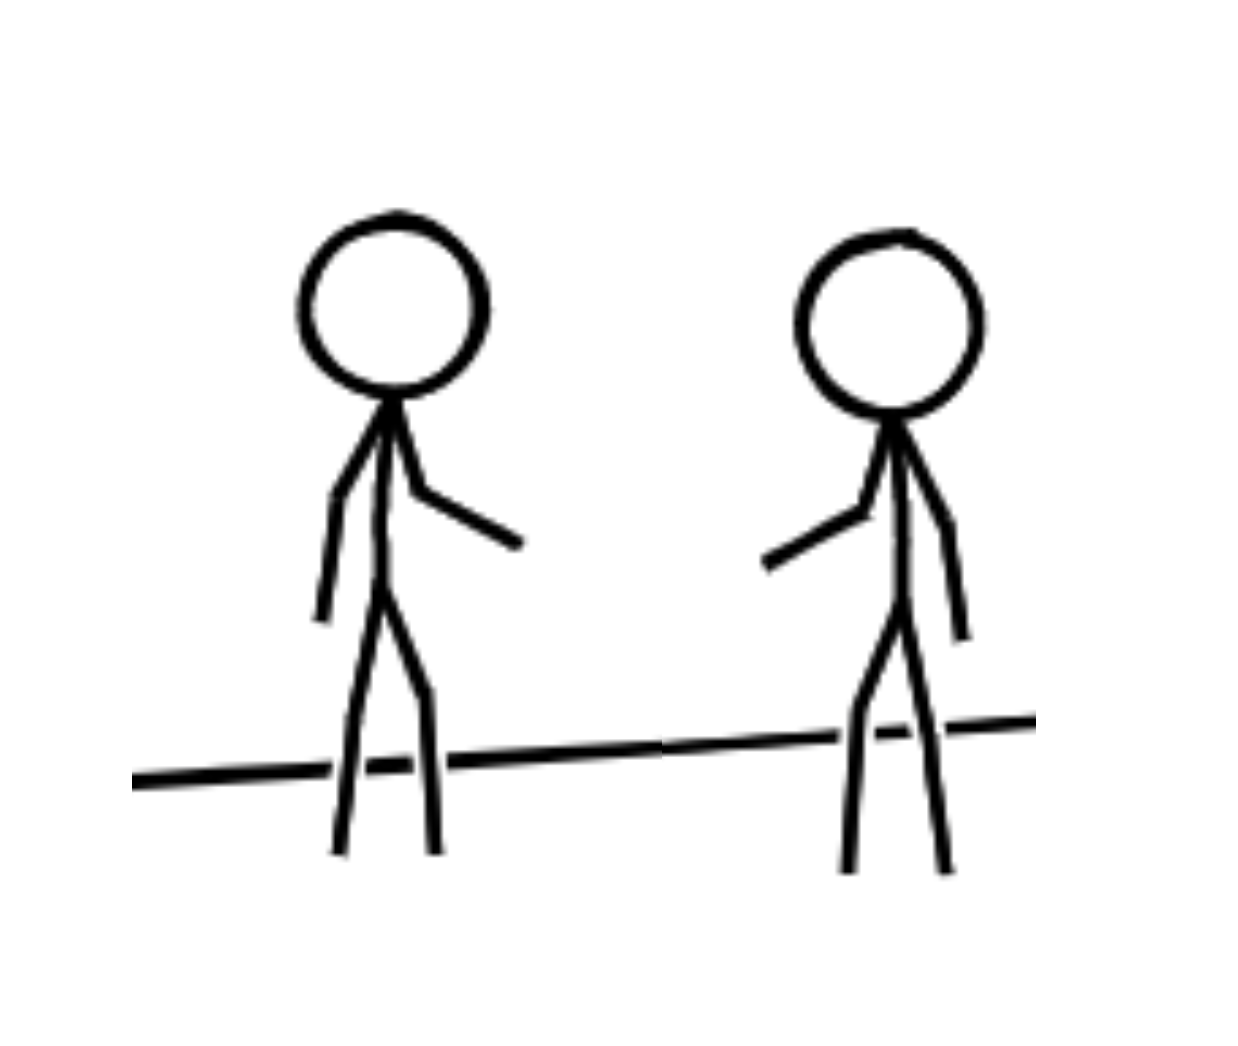
\includegraphics[width=0.3\columnwidth]{figures/xkcd_example}
  \caption{A example of abstract comic figure in XKCD style}
  \label{fig:xkcd}
\end{figure}

As a form of art, the creation of comics has few limitation. Although there is no common template that could describe all comics, if we take a closer look at each comic, it is not hard to see that every comic consists of several fundamental components. We categorize key comic elements into three groups: 1) character gestures, 2) inter-character distance, 3) background shading. To represent a persuasive message in comic form, we need to determine each of those three parameters.

The gesture of a character is another important component in the comic. The gesture of a character can help reader to understand what happens and the emotion of the character. Different gestures also imply different level of emotion intensity. As a common technique, cartoonists often use the gesture to intensify the feeling that they want to communicate to the reader \cite{scott1993understanding}. In a persuasive message, the intensified emotion may make the message more memorable than a plain tone. Thus, in this study, the gesture is one of key element that we believe may impact the perceived persuasiveness of a persuasive comic.

Beside the gesture of the character, the relationship between characters is also important. In real world, previous research suggests that messages are more persuasive if the person communicating the ideas is someone the receiver relates \cite{daddis2008influence,merga2014peer,shin2013user}. People are more likely to be influenced by their close friends than strangers. In abstract comics, the relationship between characters is usually modeled by the distance between characters \cite{scott1993understanding}. So, it is reasonable to believe the link still holds in the world of comics as the reader tends to project his/herself onto the character.

A rich body of research has demonstrated the relationship between background shading and the emotion in comics \cite{scott1993understanding}. Align with the idea of increasing memorability, representations with strong emotion can make the message more unique and memorable.

RQ3: Does different elements in a persuasive comic affect its perceived persuasiveness?
